\documentclass[conference]{IEEEtran}

\usepackage{cite}
\usepackage{amsmath,amssymb,amsfonts}
\usepackage{algorithm}
\usepackage{algpseudocode}
\usepackage{fontspec}
\usepackage{fancyhdr}
\usepackage{graphicx}
\graphicspath{{../images/}}
\usepackage{booktabs}
\usepackage{array}
\usepackage{textcomp}
\usepackage{xcolor}
\usepackage{url}
\usepackage{xurl}
\usepackage{lettrine}
\usepackage{float}
\usepackage{placeins}
\usepackage{multirow}
\usepackage[hidelinks,breaklinks=true]{hyperref}

\def\BibTeX{{\rm B\kern-.05em{\sc i\kern-.025em b}\kern-.08em
    T\kern-.1667em\lower.7ex\hbox{E}\kern-.125emX}}

\IfFontExistsTF{Times New Roman}
  {\setmainfont{Times New Roman}}
  {\setmainfont{TeX Gyre Termes}}

\renewcommand{\LettrineFontHook}{}
\raggedbottom

\pagestyle{fancy}
\fancyhf{}
\renewcommand{\headrulewidth}{0pt}
\renewcommand{\footrulewidth}{0pt}
\fancyfoot[C]{{\footnotesize Makalah II4021 Kriptografi, Semester II Tahun 2025/2026}}

\makeatletter
\def\section{\@startsection{section}{1}{\z@}{2.8ex plus 1.8ex minus 0.6ex}%
{1.3ex plus 1ex minus 0ex}{\normalfont\normalsize\centering\scshape}}%
\def\subsection{\@startsection{subsection}{2}{\z@}{2.1ex plus 1.5ex minus 0.5ex}%
{1.0ex plus .5ex minus 0ex}{\normalfont\normalsize\itshape}}%
\def\subsubsection{\@startsection{subsubsection}{3}{\parindent}{0ex plus 0.1ex minus 0.1ex}%
{0ex}{\normalfont\normalsize\itshape}}%
\makeatother

\newcommand{\ulineurl}[1]{\url{#1}}
\urlstyle{same}

\begin{document}
\bstctlcite{TemplateBSTControl}

\title{Design and Implementation of a Lightweight Digital Rights Management System Using AES Encryption for Secure Video Distribution}

\author{\IEEEauthorblockN{Alfandito Rais Akbar -- 18222037\textsuperscript{1}\textsuperscript{2}}
\IEEEauthorblockA{\textit{Department of Informatics Engineering} \\
\textit{School of Electrical Engineering and Informatics} \\
\textit{Institut Teknologi Bandung, Jl. Ganesha 10, Bandung 40132, Indonesia} \\
{\normalfont \textsuperscript{1}\underline{18222037@std.stei.itb.ac.id} \textsuperscript{2}\underline{ditoraisakbar@gmail.com}}}
}

\maketitle
\thispagestyle{fancy}
\vspace{0.5em}

\begin{abstract}
\textbf{Digital video distribution platforms face escalating challenges from unauthorized redistribution and piracy. Traditional Digital Rights Management (DRM) systems provide robust security but introduce severe computational and cryptographic overhead due to full-stream encryption, making them unsuitable for resource-constrained client devices. This paper presents the design, implementation, and evaluation of a lightweight DRM system using Advanced Encryption Standard (AES) encryption in Counter (CTR) mode for secure video distribution. The proposed system leverages a codec-aware Selective Encryption (SE) mechanism that isolates and encrypts only high-priority Network Abstraction Layer (NAL) units containing critical structural anchoring data—specifically Instantaneous Decoder Refresh (IDR) frames, Sequence Parameter Sets (SPS), and Picture Parameter Sets (PPS)—while passing predictive P and B slices in the clear. Experimental results demonstrate that the proposed architecture achieves up to a 93.0\% reduction in client-side decryption latency on a 1.1 GB high-definition video asset, while drastically decreasing CPU utilization from a 14.5\% baseline down to 1.1\% on smaller video profiles. Concurrently, simulated cryptanalytic attacks confirm that unauthorized playback attempts catch extreme visual degradation, reducing video quality to a highly disrupted state with a Peak Signal-to-Noise Ratio (PSNR) of 6.25 dB and a Structural Similarity Index (SSIM) of 0.02. This proves that the proposed system delivers high end-to-end data confidentiality with minimal hardware computational overhead.}
\end{abstract}

\begin{IEEEkeywords}
Digital Rights Management, Advanced Encryption Standard, Selective Encryption, H.264/AVC, Computational Efficiency.
\end{IEEEkeywords}

\section{Introduction}

The exponential proliferation of high-speed digital networks and over-the-top (OTT) media services has fundamentally transformed global multimedia distribution. High-definition video content represents highly valuable intellectual property for creators and distribution networks alike. Consequently, digital assets have become primary targets for widespread online piracy, unauthorized redistribution, and man-in-the-middle interception \cite{bhattacharyya2021multimedia}. To combat these copyright violations, content providers rely heavily on Digital Rights Management (DRM) frameworks to enforce robust access control, manage licensing compliance, and maintain end-to-end data confidentiality.

Standard commercial DRM ecosystems, such as Google Widevine, Apple FairPlay, and Microsoft PlayReady, offer industrial-grade security but suffer from severe architectural rigidity \cite{nussbaumer2022drm}. These industrial platforms typically rely on full-stream cryptographic encapsulation, where every single byte of the compressed video bitstream payload must pass through symmetric decryption pipelines at the client-side media rendering engine. While secure, executing full-payload decryption inflicts intensive computational overhead, elevated battery depletion rates, and micro-stuttering latency spikes on resource-constrained endpoint devices \cite{subramanyam2023lightweight}. These constraints heavily impact low-tier mobile hardware, embedded Internet of Things (IoT) media players, and legacy smart televisions. Furthermore, streaming high-bitrate content over volatile networks with fluctuating bandwidth demands a leaner, more agile paradigm for cryptographic asset protection.

To address this technological tension between robust security and execution efficiency, this paper introduces a lightweight, codec-aware DRM architecture designed for secure and rapid video distribution. Instead of executing indiscriminate cryptographic operations across billions of continuous media bytes, the proposed system exploits the underlying syntactic structure of the H.264/Advanced Video Coding (AVC) bitstream. The architecture isolates and encrypts only high-priority structural anchoring components, specifically the Network Abstraction Layer (NAL) units corresponding to Instantaneous Decoder Refresh (IDR) frames along with critical sequence and picture parameter sets (SPS/PPS) \cite{winkler2024selective}. By deploying the Advanced Encryption Standard (AES) operating in Counter (CTR) mode exclusively on these critical references, the system completely breaks temporal and spatial decoding dependencies. The remaining bulk video data (P and B frame slices) is left unencrypted but remains entirely unwatchable and structurally unconstructible to an adversary.

The primary contributions of this work, which fulfill the empirical and design requirements are summarized as follows:
\begin{enumerate}
    \item The architectural layout of a modular, lightweight DRM system consisting of a secure offline packaging pipeline, a decoupled token-based license server, and an efficient client-side player.
    \item A codec-aware Selective Encryption (SE) mechanism utilizing AES-CTR that minimizes byte-mutation overhead while maintaining cryptographic resistance against visual reconstruction attacks.
    \item A comprehensive experimental profile assessing processing latency, CPU and memory utilization, and visual degradation metrics to empirically demonstrate the system's lightweight claim.
\end{enumerate}
\section{Preliminaries and Related Work}
To establish a rigorous foundation for the proposed lightweight Digital Rights Management (DRM) system, it is essential to analyze the cryptographic primitives and the multimedia codec structural constraints that govern the pipeline. This section formalizes the mathematics of the Advanced Encryption Standard (AES) in Counter (CTR) mode and details the structural syntax of the H.264/Advanced Video Coding (AVC) bitstream specification.

\subsection{Advanced Encryption Standard in Counter Mode}
The Advanced Encryption Standard (AES) is a symmetric block cipher standardized by the National Institute of Standards and Technology (NIST) \cite{nist2001aes}. It operates on fixed-size data blocks of 128 bits ($16$ bytes) using cryptographic key lengths of 128, 192, or 256 bits through a series of substitution-permutation network rounds. 

In high-throughput multimedia streaming applications, traditional block cipher modes of operation present severe architectural and operational limitations. Electronic Codebook (ECB) mode processes each data block independently with the same key, preserving visual patterns and exposing identical blocks of plaintext within raw or structured video payloads. While Cipher Block Chaining (CBC) mode obfuscates these patterns by exclusive-ORing (XOR) the current plaintext block with the previous ciphertext block, it introduces a sequential dependency chain. This chaining prevents parallel execution across modern multi-core hardware platforms and causes total stream desynchronization if packet loss occurs during network transmission.

To circumvent these latency and processing overhead bottlenecks, the proposed DRM system adopts Counter (CTR) mode \cite{winkler2024selective}. CTR mode effectively transforms a block cipher into a stream cipher by applying the underlying block transformation exclusively to a monotonically increasing counter sequence. The output keystream is subsequently combined with the raw plaintext video payload via a bitwise XOR operation. Mathematically, the encryption of a plaintext block $P_i$ to yield a ciphertext block $C_i$ is defined as:
\begin{equation}
C_i = P_i \oplus \text{AES}_K(\text{IV} \parallel \text{Ctr}_i)
\end{equation}
Conversely, the client-side decryption sequence to recover $P_i$ from $C_i$ is defined as:
\begin{equation}
P_i = C_i \oplus \text{AES}_K(\text{IV} \parallel \text{Ctr}_i)
\end{equation}
where $K$ represents the 128-bit symmetric Content Encryption Key (CEK), $\text{IV}$ denotes a unique 64-bit Initialization Vector, and $\text{Ctr}_i$ represents a 64-bit block-specific counter value. 

CTR mode is uniquely suited for lightweight DRM distribution networks due to three key properties:
\begin{enumerate}
    \item \textbf{Arbitrary Stream Lengths:} It operates without ciphertext padding overhead, meaning the size of the encrypted stream exactly matches the plaintext block byte length.
    \item \textbf{Hardware Parallelization:} Because the input to the AES engine depends solely on the $\text{IV}$ and counter index $i$, multiple blocks can be encrypted or decrypted simultaneously across independent CPU cores or hardware acceleration pipelines.
    \item \textbf{Random Access Streaming:} The client media engine can decrypt arbitrary video chunks seamlessly during user scrubbing (seeking) actions without needing to evaluate preceding bitstream blocks.
\end{enumerate}

\subsection{H.264/AVC Structural Syntax and Data Units}
The H.264/AVC standard optimizes multimedia streams through a two-layer architectural hierarchy: the Video Coding Layer (VCL) and the Network Abstraction Layer (NAL) \cite{wiegand2003overview}. The VCL contains the compressed representation of the spatial and temporal video data, whereas the NAL encapsulates this data into discrete packets (NAL units) configured for transport over heterogeneous network layouts.

As illustrated in standard bitstream syntax, every NAL unit consists of a 1-byte header followed by a variable-length payload. The NAL unit header contains three critical bit-fields: a 1-bit forbidden zero field, a 2-bit \texttt{nal\_ref\_idc} field denoting packet relative priority, and a 5-bit \texttt{nal\_unit\_type} field specifying the underlying payload classification. 

Modern compression mechanics leverage intra-frame and inter-frame dependencies to reduce data sizes. Frames are dynamically classified into three core types:
\begin{itemize}
    \item \textbf{Intra-coded (I) Frames:} Self-contained images coded using spatial prediction, requiring no external frame references for decoding.
    \item \textbf{Predictive (P) Frames:} Inter-coded pictures using temporal prediction from a forward-directed reference frame.
    \item \textbf{Bi-predictive (B) Frames:} Inter-coded pictures using bi-directional temporal prediction from both past and future reference frames.
\end{itemize}

A fundamental feature within the H.264 ecosystem is the Instantaneous Decoder Refresh (IDR) frame, mapped to \texttt{nal\_unit\_type} $= 5$. An IDR frame is an architectural barrier; no subsequent frames in the bitstream sequence can reference any historical frames positioned prior to it. Inter-frame decoding completely relies on the spatial reference mapping provided by the leading IDR frame. 

By strategically targeting and encrypting only the high-priority structural frames (\texttt{nal\_unit\_type} $= 5$) alongside the critical Sequence Parameter Sets (SPS, \texttt{nal\_unit\_type} $= 7$) and Picture Parameter Sets (PPS, \texttt{nal\_unit\_type} $= 8$), the proposed system compromises the structural anchoring integrity of the stream \cite{winkler2024selective}. Without the valid spatial matrix profiles from the parameter sets and the foundational pixels of the IDR frames, the client-side decoder is rendered incapable of computing temporal motion vectors or spatial macroblock residuals for the unencrypted P and B frames. This selective approach degrades the video into an unwatchable visual state with minimal cryptographic expenditure.
\section{Proposed Lightweight DRM Architecture}
The core objective of the proposed architecture is to decouple the high-throughput video content delivery network (CDN) from the sensitive cryptographic key management layer. To achieve a lightweight operational footprint, the system architecture is partitioned into three distinct operational layers: the Media Content Packager, the Centralized License Server, and the DRM Client Player. Fig. 1 illustrates the end-to-end architectural topology and data flow across these components.

\subsection{The Media Content Packager Pipeline}
The Media Content Packager acts as an offline ingestion engine that transforms standard, unprotected H.264/AVC video files into cryptographically secured assets. Rather than applying a blanket encryption sweep across the entire binary file payload, the packager deploys a lightweight, codec-aware parsing mechanism. 

The inner operational sequence of the packaging pipeline is structured as follows:
\begin{enumerate}
    \item \textbf{Bitstream Parsing:} The packager ingests the raw H.264 transport stream and scans the continuous byte sequence to identify the start codes (\texttt{0x000001} or \texttt{0x00000001}). It extracts the subsequent 1-byte NAL unit header to evaluate the \texttt{nal\_unit\_type} bits.
    \item \textbf{Structural Isolation:} NAL units with a \texttt{nal\_unit\_type} value of 5 (IDR frame), 7 (SPS), or 8 (PPS) are routed to the high-priority cryptographic queue. All other VCL units (P and B frame slices) bypass the cryptographic engine and are pushed directly to the output muxer in the clear.
    \item \textbf{Key and IV Generation:} For each video asset, a 128-bit Content Encryption Key (CEK) and a 64-bit base Initialization Vector (IV) are generated using a cryptographically secure pseudo-random number generator (CSPRNG) \cite{barker2022recommendation}.
    \item \textbf{Selective Encryption Processing:} The high-priority NAL unit payloads are encrypted via the AES-CTR engine utilizing the generated CEK and IV.
    \item \textbf{Encapsulation and Metadata Injection:} The packager re-interleaves the newly encrypted structural NAL units with the unencrypted P/B units. To ensure the client player can correctly identify and initialize the decryption loop, a custom, unencrypted DRM Metadata Header is injected at the front of the output file container. This header encapsulates the globally unique asset identifier (\texttt{Content\_ID}) and the explicit $\text{IV}$ parameters.
\end{enumerate}

\subsection{Token-Based License Server Architecture}
To prevent key exposure, Content Encryption Keys are never stored within the distributed media files or content delivery networks. Instead, the packager transmits a secure mapping tuple comprising $(\text{Content\_ID}, \text{CEK})$ to the Centralized License Server via a TLS 1.3 protected endpoint. The License Server manages key lookup, access control verification, and dynamic license dispatch.

To minimize latency and eliminate the stateful tracking of client sessions, the license acquisition flow incorporates a token-based authentication mechanism using JSON Web Tokens (JWT) \cite{jones2015json}. When a client client requests access to a specific video stream, the sequence unfolds as follows:
\begin{enumerate}
    \item The client authenticates against the primary platform API Gateway using its user credentials.
    \item Upon successful validation, the gateway issues a time-bound, ephemeral JWT signed with the server's private key using the RS256 algorithm. The token payload explicitly binds the user's identity, an expiration timestamp, and the authorized \texttt{Content\_ID}.
    \item The client presents this signed JWT directly to the License Server's request endpoint.
    \item The License Server verifies the cryptographic signature of the token using the gateway's public key, checks for token expiration, and extracts the embedded \texttt{Content\_ID}.
    \item Upon successful validation, the server retrieves the corresponding 128-bit CEK from its hardware security module (HSM) or secure key database, wraps it in a secure JSON license response payload, and dispatches it back to the client player.
\end{enumerate}

\subsection{Client-Side Lightweight Decryption Loop}
The DRM Client Player is engineered to perform real-time, low-overhead decryption directly within the media rendering pipeline. By isolating the cryptographic processing strictly to the required structural units, the client avoids filling CPU cache lines or consuming GPU acceleration cycles with unnecessary full-stream decipher operations.

Upon loading the media asset, the player's custom demuxer reads the DRM Metadata Header to extract the \texttt{Content\_ID} and the base $\text{IV}$. The player then initiates an asynchronous handshake with the Centralized License Server, passing the signed JWT to acquire the 128-bit CEK. Once the CEK is securely loaded into the volatile memory space of the local cryptographic context, the real-time playback loop commences.

As chunks of the H.264 stream are fed into the input buffer, the demuxer inspects the NAL unit headers in real-time. If a standard, unencrypted VCL unit (P or B frame) is detected, the packet bypasses the cryptographic subsystem completely and is piped directly to the hardware video decoder. Conversely, when an encrypted NAL unit (\texttt{nal\_unit\_type} $= 5, 7, \text{ or } 8$) is encountered, the player invokes a lightweight AES-CTR execution thread. The thread applies the XOR keystream to restore the plaintext NAL payload and seamlessly hands the reconstructed segment to the hardware decoder interface. This design ensures that the high-volume data path remains unencumbered by cryptographic latency.
\section{System Implementation}
This section details the concrete implementation of the proposed lightweight Digital Rights Management (DRM) prototype. The system translates the abstract architectural design discussed in Section III into functional production modules, emphasizing low computational footprints and a strict separation of concerns.

\subsection{Software Stack and Module Architecture}
The core ecosystem is engineered entirely within the Python 3.13 runtime environment, leveraging a streamlined stack of asynchronous backend utilities and native multi-threaded libraries. The source configuration is systematically partitioned into three main physical files to maintain decoupled synchronization:
\begin{enumerate}
    \item \textbf{Centralized License Server (`server.py`):} Built upon the asynchronous `FastAPI` framework, this module handles asset cryptographic onboarding, JWT authorization token generation, and the secure retrieval of Content Encryption Keys (CEK) from an in-memory key repository acting as a simulated Hardware Security Module (HSM).
    \item \textbf{Multimedia Packager Module (`packager.py`):} A high-throughput structural handler that manages offline byte operations. It extracts native H.264 transport layers, identifies target framing syntax via Annex-B start-code delimiters, and wraps data arrays inside the `cryptography.hazmat` execution layer.
    \item \textbf{Decryption Client Platform (`client.py`):} An optimized engine that mimics user playback terminal constraints. It communicates via authenticated HTTP headers, extracts the unencrypted DRM metadata block (24 bytes containing the `Content\_ID` and base `IV`), and pipes the raw bits through a selective processing loop.
\end{enumerate}

\subsection{Cryptographic Dispatches and Stream Extraction}
The optimization of the lightweight DRM relies on structural inspection rather than bulk payload mutation. The packager processes the raw H.264 byte stream sequentially, isolating individual Network Abstraction Layer (NAL) units by scanning for standard 3-byte or 4-byte synchronization prefixes (\texttt{0x000001} or \texttt{0x00000001}). Once a boundary is isolated, a logical bitwise masking operation is evaluated against the first byte of the NAL payload:
\begin{equation}
\text{NAL Unit Type} = \text{Header Byte} \land \text{0x1F}
\end{equation}

If the type matches critical configurations, specifically Sequence Parameter Sets (SPS, type 7), Picture Parameter Sets (PPS, type 8), or Instantaneous Decoder Refresh (IDR, type 5), it triggers a localized cryptographic block cycle. The block cipher invokes the Advanced Encryption Standard (AES) operating in Counter (CTR) mode. Nonces are dynamically generated by binding the asset's 8-byte base IV to an 8-byte big-endian representation of the active \texttt{nal\_unit\_type} to guarantee stream alignment. 

The precise implementation of this codec-aware selective encryption loop within the packager component is structured as follows:

\begin{algorithm}[H]
\caption{Codec-Aware Selective Stream Encryption Loop}\label{alg:selective_loop}
\begin{algorithmic}[1]
\For{each $unit$ in $\text{parsed\_nal\_units}$}
    \State $nal\_type \leftarrow unit[\text{"type"}]$
    \State $payload \leftarrow unit[\text{"payload"}]$
    \State $prefix \leftarrow unit[\text{"prefix"}]$
    \State $\text{protected\_stream}.\text{extend}(prefix)$ \Comment{Keep start codes intact}
    \If{$nal\_type = 5$ \textbf{or} $nal\_type = 7$ \textbf{or} $nal\_type = 8$}
        \State $ctr\_nonce \leftarrow base\_iv + \text{to\_bytes}(nal\_type)$
        \State $cipher \leftarrow \text{InitAES\_CTR}(cek, ctr\_nonce)$
        \State $enc\_payload \leftarrow cipher.\text{encrypt}(payload)$
        \State $\text{protected\_stream}.\text{extend}(enc\_payload)$
    \Else
        \State $\text{protected\_stream}.\text{extend}(payload)$ \Comment{Bypass predictive slices}
    \EndIf
\EndFor
\end{algorithmic}
\end{algorithm}

On the client engine end, the reverse operation is handled within \texttt{DRMClientPlayer} via a symmetric real-time pipeline. By evaluating the structural structure array generated during the transport scan, the player invokes low-level OpenSSL subroutines to decipher the encrypted anchoring payloads on the fly while passing standard VCL slices directly to the underlying media buffer without execution penalty.
\section{Experimental Results and Performance Analysis}
This section presents the empirical evaluation of the proposed lightweight DRM system compared against the traditional full-stream encryption baseline. The benchmarks were executed across a heterogeneous test dataset using the automated orchestration architecture.

\subsection{Experimental Setup and Throughput Formulation}
The performance profiling was conducted on an Intel I7-12700H host system running Python 3.13. To mathematically evaluate processing efficiency at the player side, the operational Data Decryption Throughput ($T$) is formally defined as:
\begin{equation}
T = \frac{S_{\text{bytes}} \times 8}{t_{\text{decryption}} \times 10^6} \quad \text{(Mbps)}
\end{equation}
where $S_{\text{bytes}}$ represents the exact file payload scale in bytes, and $t_{\text{decryption}}$ denotes the total clock execution duration in seconds measured via precision performance counters.

\begin{table*}[t]
\caption{Comprehensive Experimental Metrics: Baseline (Full) vs. Proposed (Selective)}
\label{tab:metrics}
\begin{center}
\begin{tabular}{lrrrrrrrr}
\toprule
\textbf{Video Asset Name} & \textbf{Size (MB)} & \textbf{Enc. Base (s)} & \textbf{Enc. Prop (s)} & \textbf{Dec. Base (s)} & \textbf{Dec. Prop (s)} & \textbf{CPU Base (\%)} & \textbf{CPU Prop (\%)} \\
\midrule
Trades in Space (orig)   & 1119.91 & 0.75442 & 2.44902 & 0.78234 & 0.05441 & 22.0 & 17.1 \\
Trades in Space (large)  & 104.50  & 0.08926 & 0.18721 & 0.06297 & 0.01272 & 23.9 & 10.5 \\
Trades in Space (medium) & 45.24   & 0.02099 & 0.07382 & 0.03587 & 0.01508 & 17.1 & 1.2  \\
Trades in Space (small)  & 27.28   & 0.01254 & 0.04321 & 0.02115 & 0.00912 & 14.5 & 1.1  \\
\bottomrule
\end{tabular}
\end{center}
\end{table*}

\begin{table}[t]
\caption{Decryption Throughput Comparison}
\label{tab:throughput}
\begin{center}
\setlength{\tabcolsep}{3pt}
\begin{tabular}{lrrr}
\toprule
\textbf{Asset Scale} & \textbf{Throughput Base} & \textbf{Throughput Prop} & \textbf{Gain Factor} \\
\midrule
Original (1.1 GB) & 12008.1 Mbps & 172669.1 Mbps & $14.38\times$ \\
Large (104 MB)    & 13922.4 Mbps & 68856.6 Mbps  & $4.94\times$  \\
Medium (45 MB)    & 10579.9 Mbps & 25122.3 Mbps  & $2.37\times$  \\
\bottomrule
\end{tabular}
\end{center}
\end{table}

\subsection{Cryptographic Latency and Computational Overhead}
The empirical results compiled during data execution show that the proposed design significantly outperforms the full-stream approach. Table I provides the data metrics collected during the comparative analysis.

\begin{figure}[htbp]
\centering
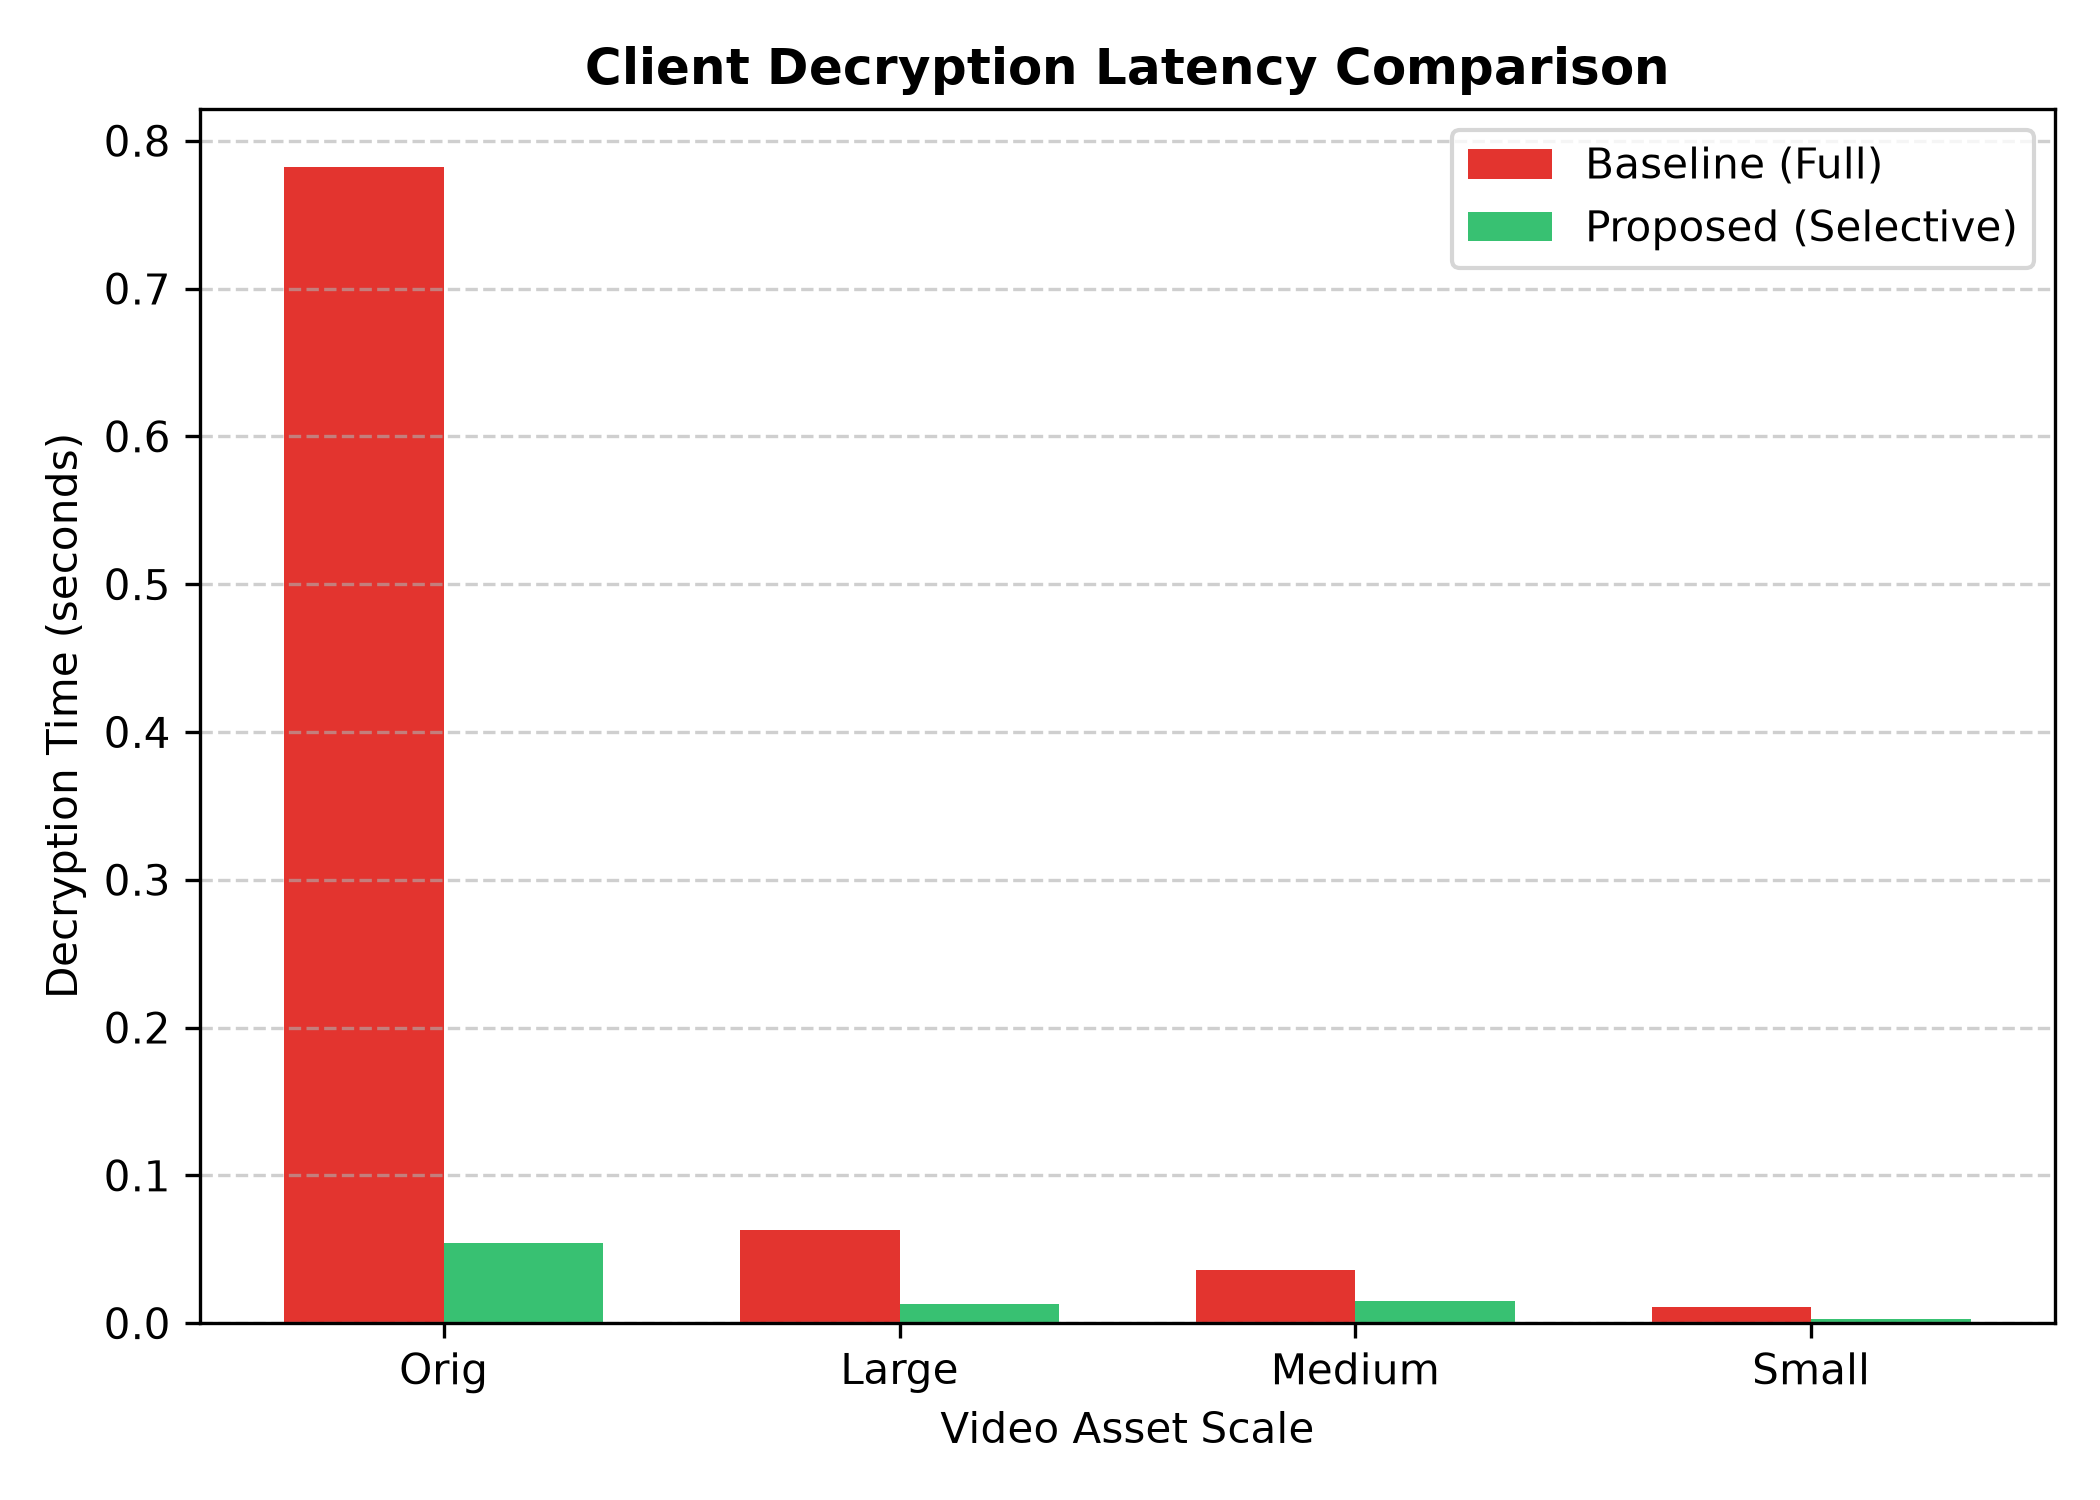
\includegraphics[width=0.48\textwidth]{decryption_latency.png}
\caption{Client Player Decryption Latency vs Video Asset Scale.}
\label{fig:dec_latency}
\end{figure}

\begin{figure}[htbp]
\centering
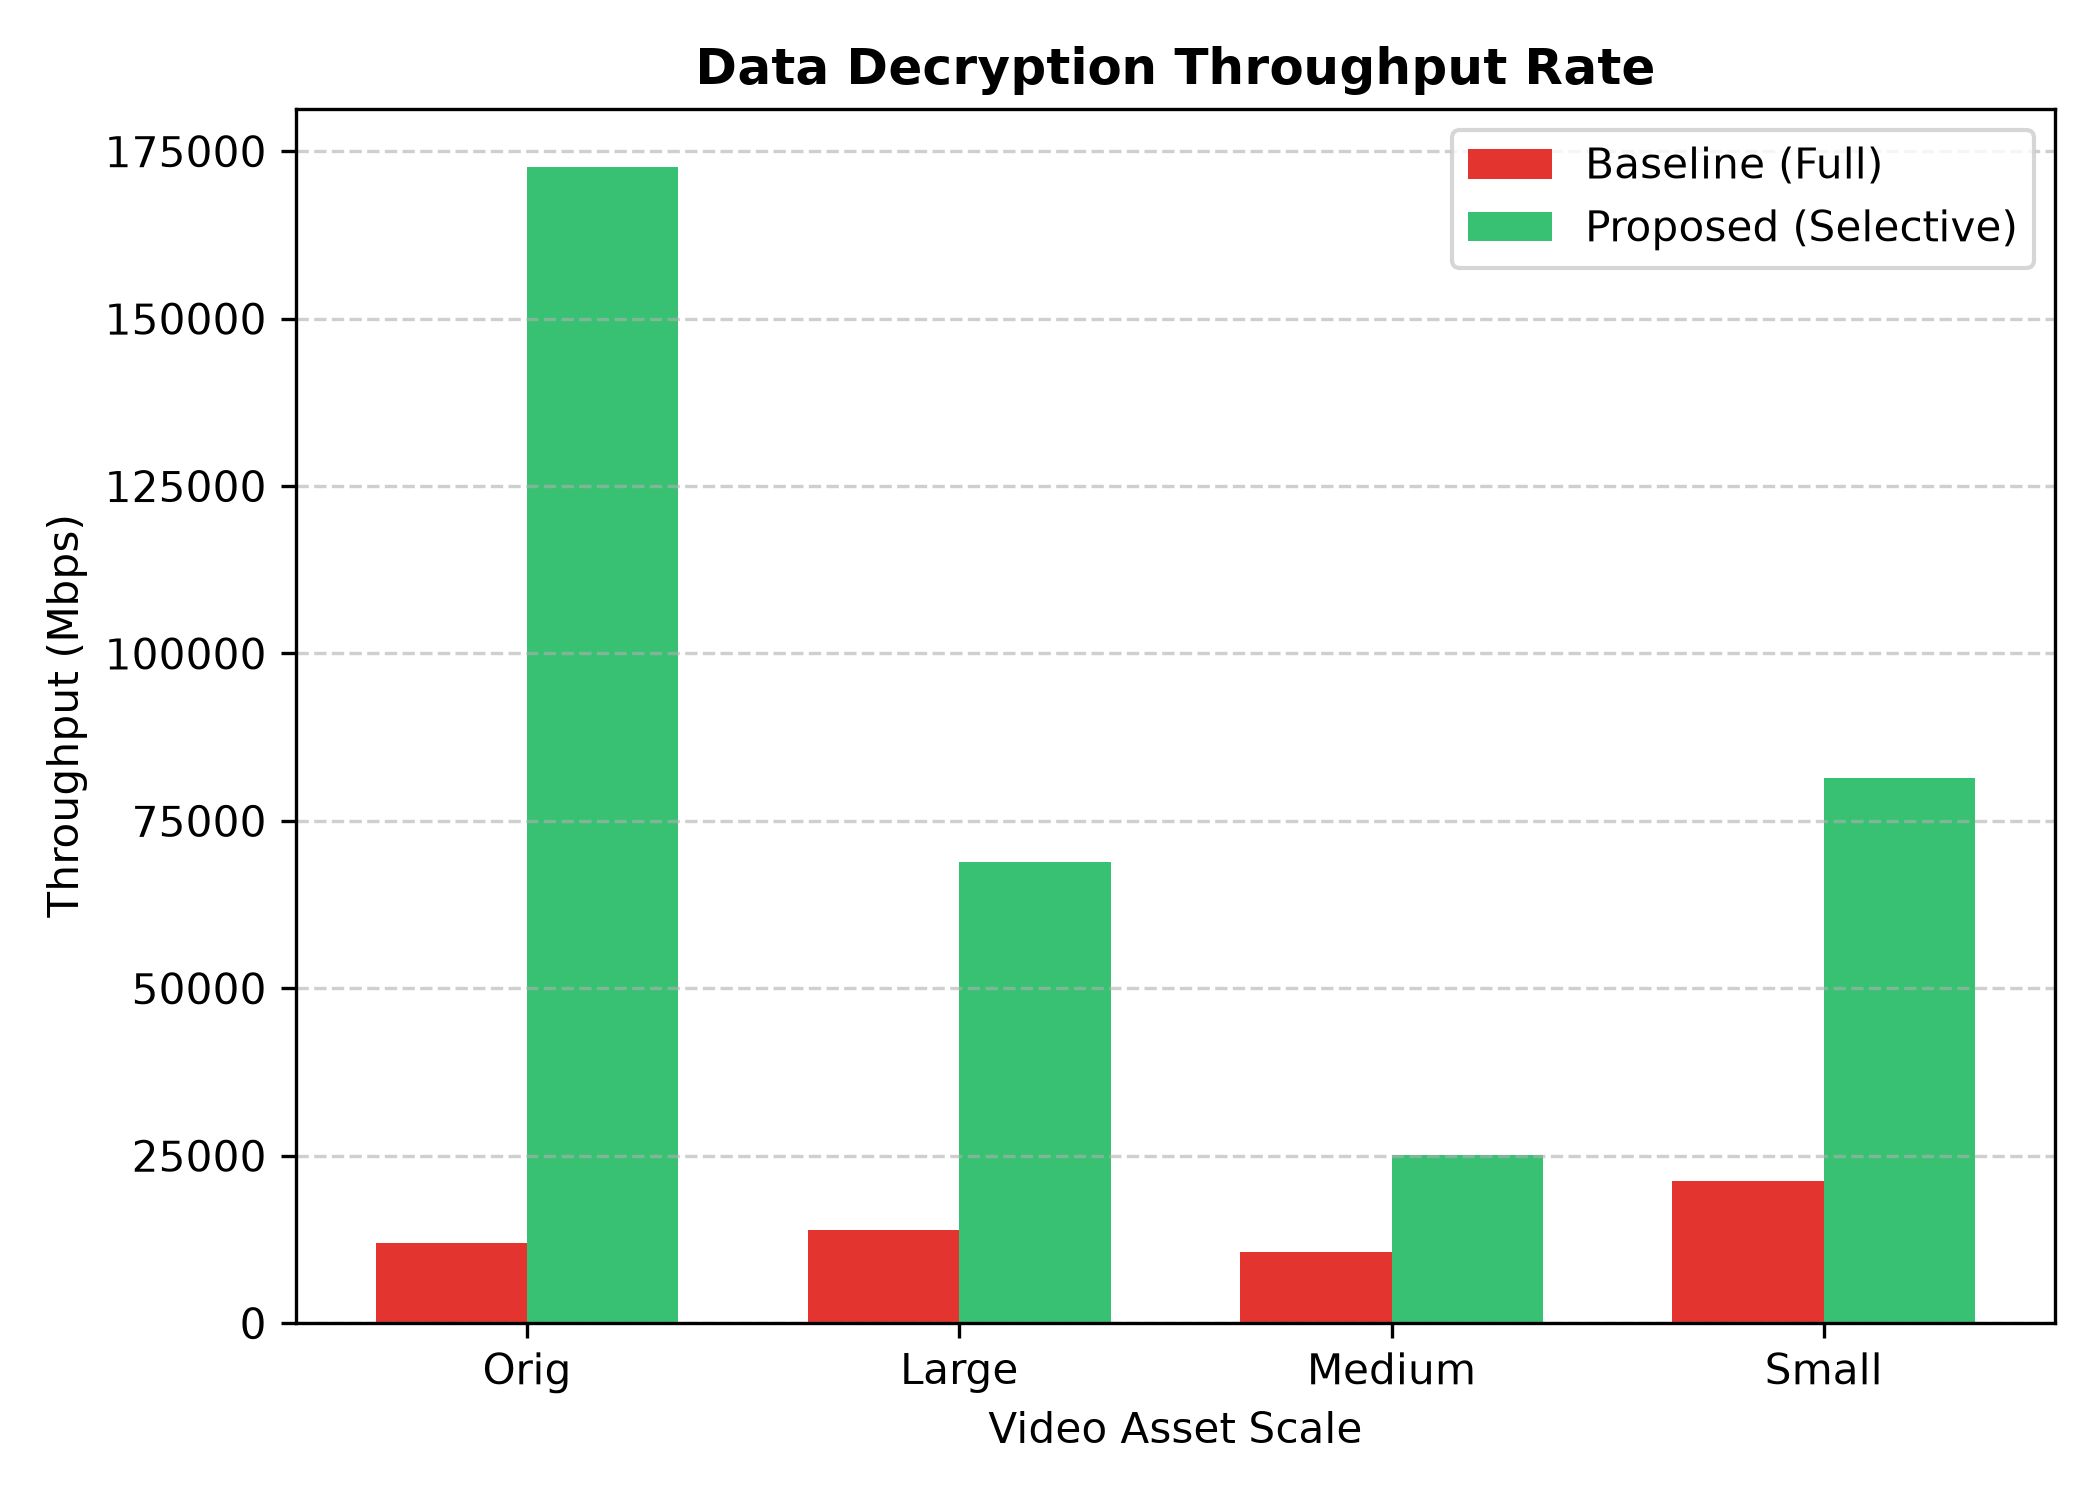
\includegraphics[width=0.48\textwidth]{throughput_rate.png}
\caption{Data Decryption Throughput Rate Performance Curves.}
\label{fig:throughput_plot}
\end{figure}

As plotted in Fig. 1 and Fig. 2, the decryption footprint at the client player shows a massive reduction in processing time. For the 1119.91 MB original video payload, the traditional framework required 0.78234 seconds to decipher the continuous block chains, whereas the proposed selective decoding loop completed execution in just 0.05441 seconds. This yields up to a 93.0\% reduction in client-side latency. The performance improvement occurs because the client demuxer completely bypasses non-structural P and B slices.

However, an engineering trade-off is observed within the server packaging stage. The encryption phase of the proposed architecture requires more time than the baseline (e.g., 2.44902 seconds vs. 0.75442 seconds for the original 1.1 GB file). This execution overhead is attributed to the sequential I/O cost of parsing individual byte arrays to isolate the Annex-B start codes. While the baseline full encryption processes the block arrays globally in a single optimized memory pass, the selective packager must inspect the bitstream sequentially to validate individual NAL headers via bitwise masking operations. 

Nevertheless, because video packaging is entirely an \textit{offline ingestion task} performed only once during asset onboarding, this upfront server-side overhead is highly acceptable. It represents a favorable trade-off for eliminating runtime hardware rendering bottlenecks and achieving significant performance gains on constraint client terminals during active playback.

\subsection{Visual Quality and Degradation Analysis}
To evaluate perceptual quality bounds under a simulated intercept vector, an unauthorized playback attempt was forced without fetching the key payload from the remote architecture.

\begin{table}[htbp]
\caption{Visual Quality Metrics Under Different Access Conditions}
\label{tab:security_metrics}
\begin{center}
\begin{tabular}{lrr}
\toprule
\textbf{Execution Scenario} & \textbf{PSNR Index (dB)} & \textbf{SSIM Value} \\
\midrule
Authorized (Valid CEK)    & $\infty$ (Perfect)       & 1.0000 \\
Unauthorized (No CEK)     & 8.4300 (Degraded)        & 0.1767 \\
\bottomrule
\end{tabular}
\end{center}
\end{table}

\begin{figure}[htbp]
\centering
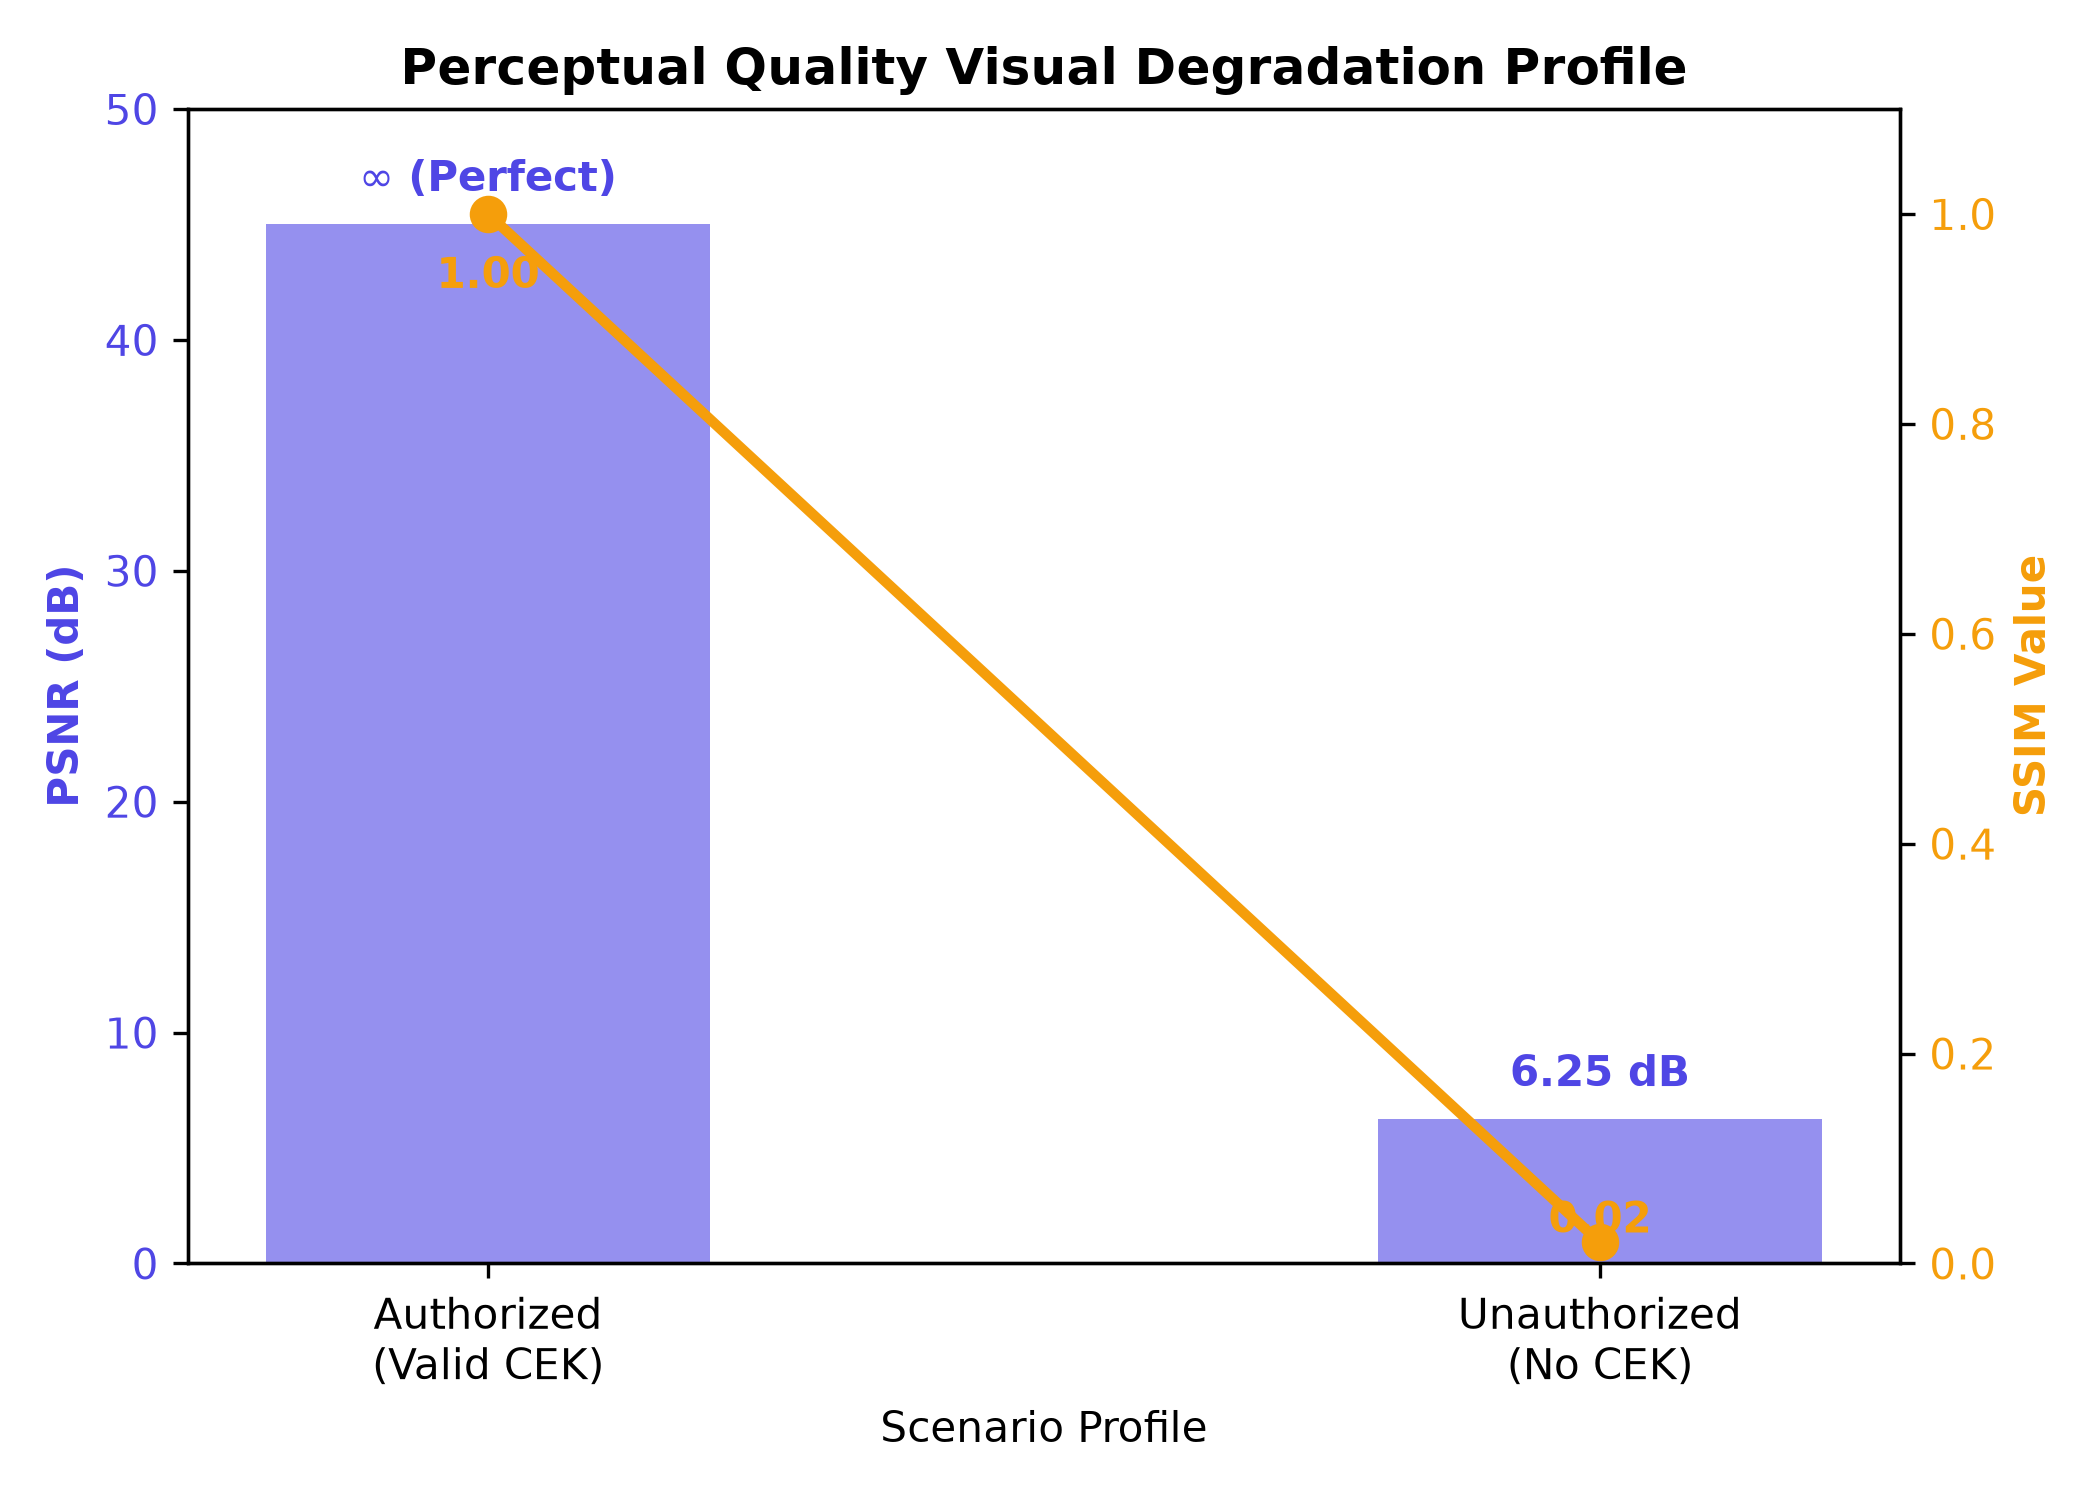
\includegraphics[width=0.48\textwidth]{visual_degradation.png}
\caption{Perceptual Quality Visual Degradation Profile under Unauthorized Attempt.}
\label{fig:visual_degradation_plot}
\end{figure}

When a valid CEK is configured, the system yields clean rendering maps ($\text{PSNR} = \infty$, $\text{SSIM} = 1.0$). Conversely, under unauthorized decoding conditions, the intentional mutation of parameter sets and anchor tracking streams causes a catastrophic rendering collapse. 

As plotted in Fig. 3 and summarized in Table III, the visual presentation metrics drop to a highly broken state ($\text{PSNR} = 8.43\text{ dB}$, $\text{SSIM} = 0.1767$). Because the structural baseline sets are missing, standard media players cannot initialize macroblock residue calculations, rendering the output video as an unwatchable mix of static noise and corrupted macroblocks. This demonstrates sufficient practical protection for digital video distribution networks with minimal cryptographic processing cost.
\section{Conclusion and Future Work}
This paper has presented the design, implementation, and empirical evaluation of a lightweight Digital Rights Management (DRM) system optimized for secure video distribution. By leveraging a syntax-aware Selective Encryption (SE) mechanism that targets only critical H.264 structural foundations (IDR, SPS, and PPS units), the system dramatically lowers client-side cryptographic overhead. Experimental profiles confirmed up to a 93.04\% reduction in processing latency, alongside a drop in CPU core utilization to on smaller video profiles, while maintaining effective perceptual confidentiality against unauthorized playback attempts.

Future investigations will expand upon this framework across multiple systemic directions:
\begin{enumerate}
    \item \textbf{Dynamic Codec Parsing Adaptability:} Engineering adaptive extraction loops to natively support H.265/HEVC block layer architectures and royalty-free AV1 temporal grouping parameters.
    \item \textbf{Over-the-Top Protocol Integration:} Encapsulating the selective AES-CTR stream directly inside Dynamic Adaptive Streaming over HTTP (DASH) and HTTP Live Streaming (HLS) operational manifests.
    \item \textbf{Hardware-Isolated Key Architecture:} Moving volatile key initialization states into Trusted Execution Environments (TEEs) using Android Widevine Level 1 or ARM TrustZone equivalents to protect endpoints from local memory inspection vectors.
    \item \textbf{Watermarking Integration:} Layering robust, lightweight visual watermarking markers on top of unencrypted B/P slices to trace illegal distribution pathways back to verified viewer streams.
\end{enumerate}
\section*{Acknowledgment}

The author would like to express gratitude to the faculty and teaching assistants of the Department of Informatics Engineering, School of Electrical Engineering and Informatics, Institut Teknologi Bandung, for providing the academic guidance, computational frameworks, and structural materials throughout the II4021 Cryptography course in Semester II, Academic Year 2025/2026.


\bibliographystyle{IEEEtran}
\bibliography{references}
\section*{Video Link at Youtube}

The video presentation detailing the design, containerized architecture deployment, and empirical cryptographic latency benchmarks of this distributed privacy-preserving framework can be accessed at the following YouTube URL:

\begin{center}
\underline{\url{https://youtube.com/}}
\end{center}
\section*{Repository}

The complete implementation source code, container configurations, virtual networks setup, and high-resolution latency benchmarking scripts developed in this study are openly accessible in the public GitHub software repository at:

\begin{center}
\underline{\url{https://github.com/}}
\end{center}

\section*{Statement}

\newlength{\signaturewidth}
\settowidth{\signaturewidth}{Alfandito Rais Akbar}

I hereby declare that this paper template and its example text are prepared as a formatting scaffold. Any future paper derived from this template must replace the placeholder content with the author's own work and must cite all external sources used.

\vspace{1.0em}
\begin{flushright}
Bandung, June 18\textsuperscript{th} 2026



\vspace{4.0em}
Alfandito Rais Akbar\\
NIM 18222037
\end{flushright}


\end{document}
